\chapter{Auswertung den Ergebnissen und kritische Auseinandersetzung}
\label{ch:Auswertung den Ergebnissen}
Anhand vorgeschlagene in dem Teil \ref{ch:Änderungen durch neue Antriebe, Annahmen und Methodik} Methodik wurde in diesem 
Kapitel den Vergleich zwischen Referenz-Flugzeugen und alternativen Antrieben geschaffen.
Außerdem werden aufgestellte Betriebsszenarien ausgewertet, schließlich diskutiert und mit anderen Arbeiten verglichenen, als auch auf die
Vorschläge für die anderen Arbeiten eingegangen.

\section{Vergleich von Referenzflugzeugen und neuen Antrieben}
\label{s:Ergebnisse_Flugzeuge}
Folgende Erkenntnisse ermöglichen Diskussion der ersten Hypothese. Die Ergebnisse sind nach Flugdistanzen aufgeteilt.\\
%
\paragraph{Kurzstreckenvergleich: Batterieantrieb und SAF vs. konventioneller Treibstoff}
%
In der Abbildung \ref{vergleichBA_Ref} sind die Ergebnisse für batteriebetriebenes ES-19 und konventionelles L410 dargestellt.
Der Vergleich wurde für 400 Kilometer Flug gemacht.
%
Die Gesamtbetriebskosten des ES-19 sind ca. 22 \% höher des konventionellen L410, wobei der Antrieb mit SAF nur 3,6 \% höher
Ergebnis liefert. Entgelte und Gebühre bewirken den größten Teil der Betriebskosten
aller verglichenen Antrieben, gefolgt von kapitalbezogenen Kosten. Bei den ersten ist einen signifikanten Unterschied zu 
konventionellem Antrieb zu sehen, 
nämlich 56 \%, bei den zweiter sind das 36 \% höhere Kosten bei BA. Der Anteil der Treibstoff- bzw. Energiekosten ist am niedrigsten 
im Vergleich zu anderen Kosten und die Treibstoffkosten sind bei konventionellem Flugzeug 30 \% höher. Die Treibstoffkosten für SAF
sind wesentlich höher (38 \%).

\begin{figure}[h]
	\centering
	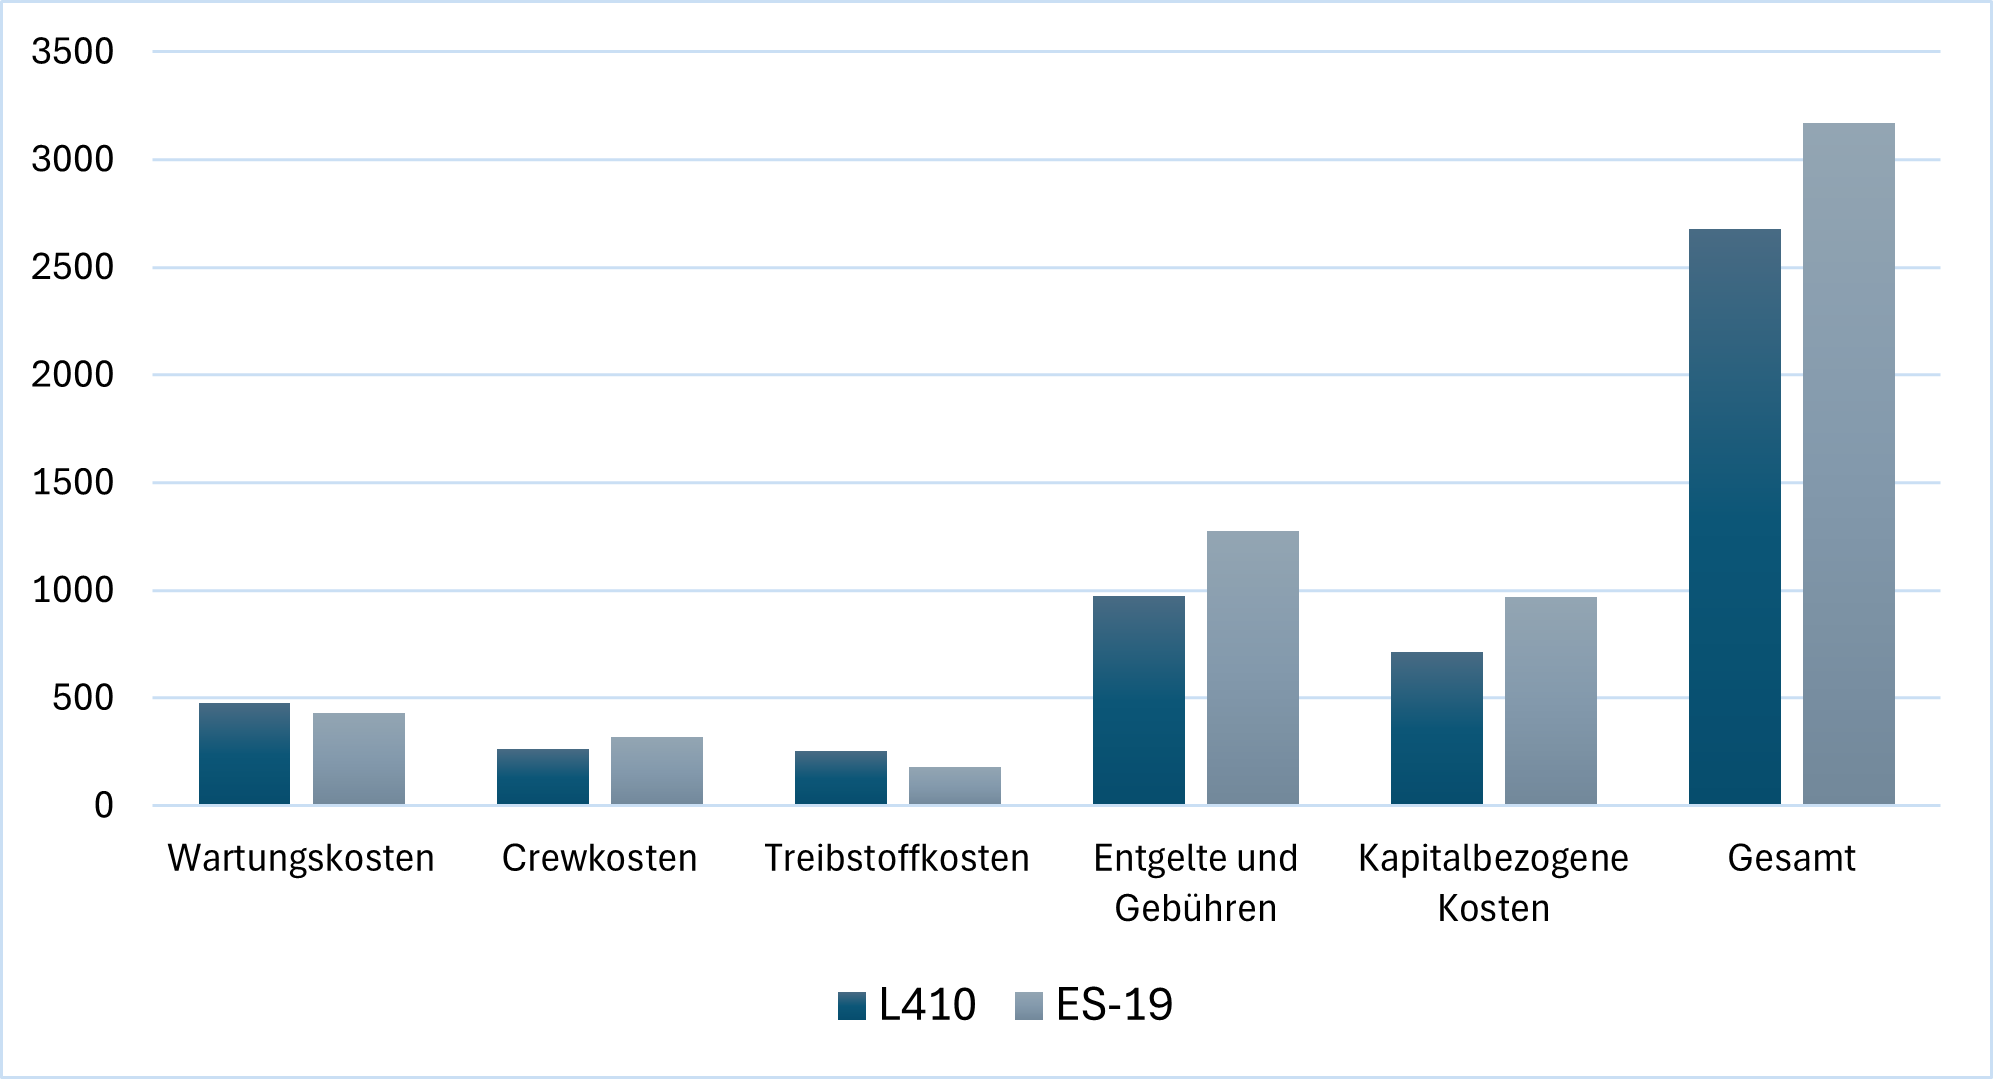
\includegraphics[width=0.9\linewidth]{Bilder/VergleichBA_Ref.png}
	\caption[Betriebskosten]{Vergleich der Referenz und Flugzeug mit der Batterie-Antrieb und SAF}
	\label{vergleichBA_Ref}
\end{figure}

Zu Entgelten und Gebühren bringen die zusätzlichen Abfertigungskosten in der Flughafenentgelte bei, wie Batteriewechsel oder Leasing der Batterie
für den Flug. Dieser Wert wird auch in der Sensitivitätsanalyse \ref{s:Sensitivitätsanalyse} überprüft. Der Einflusswert für kapitalbezogenen Kosten ist
der Anschaffungspreis von einem Flugzeug. Dieser Wert wurde als weiterer Parameter für Sensitivitätsanalyse ausgewählt.\\

\paragraph{Langstreckenvergleich: Wasserstoffantrieb und SAF vs. konventioneller Treibstoff}
In den weiteren Abschnitten wird die Gegenüberstellung zwischen den herkömmlichen Treibstoffen, SAF
und Flugzeug mit wasserstoffbetriebener Turbine für 6000 Kilometer-Flug durchgeführt. %satz übelstschlecht
Aufgrund der hohen derzeitigen Wasserstoffpreise wurde zum Vergleich der Wasserstoffmindestpreis von 2,1 $EUR/kg$ für den 
Jahr 2050 herangezogen \cite{hoelzen2022hydrogen}, um die mögliche Entwicklung der Wasserstofftechnologien zu sehen.
%
Das Ergebnis zeigt, dass die SAF- und Wasserstoffbetriebene Flugzeuge höhere Betriebskosten haben (siehe \ref{vergleichWA_Ref}).
Die Betriebskosten für Wasserstoffturbine fallen 40 \% und für SAF etwa 19 \% teurer ein.
Treibstoff- und kapitalbezogene Kosten haben den größten Einfluss auf die Gesamtkosten, Wartungs- und Crewkosten entgegen den geringsten.
Einfluss der Entgelte und Gebühren auf Gesamtkosten ist nicht so groß, wie bei dem kleineren verglichenen Flugzeugen.
Der Treibstoffkosten für WA sind fast doppelt so hoch (ca. 197 \%) wie für herkömmlichen Triebwerk. Die Entgelte und Gebühren, 
Crew- und Wartungskosten haben nicht so ein drastischer Unterschied zu konventionellen Antrieb. 
%
Werden die Entwicklung zukünftigen Preise für Wasserstoff mitbetrachtet, kann es sogar zu geringeren Treibstoffkosten im Vergleich 
zu konventionellen Antrieb führen. Die Gesamtbetriebskosten werden jedoch teurer bleiben.

%mögliche Hypothese: zukünftige Preisniveau ermöglicht die günstigere Preiswerte
\begin{figure}[h]
	\centering
	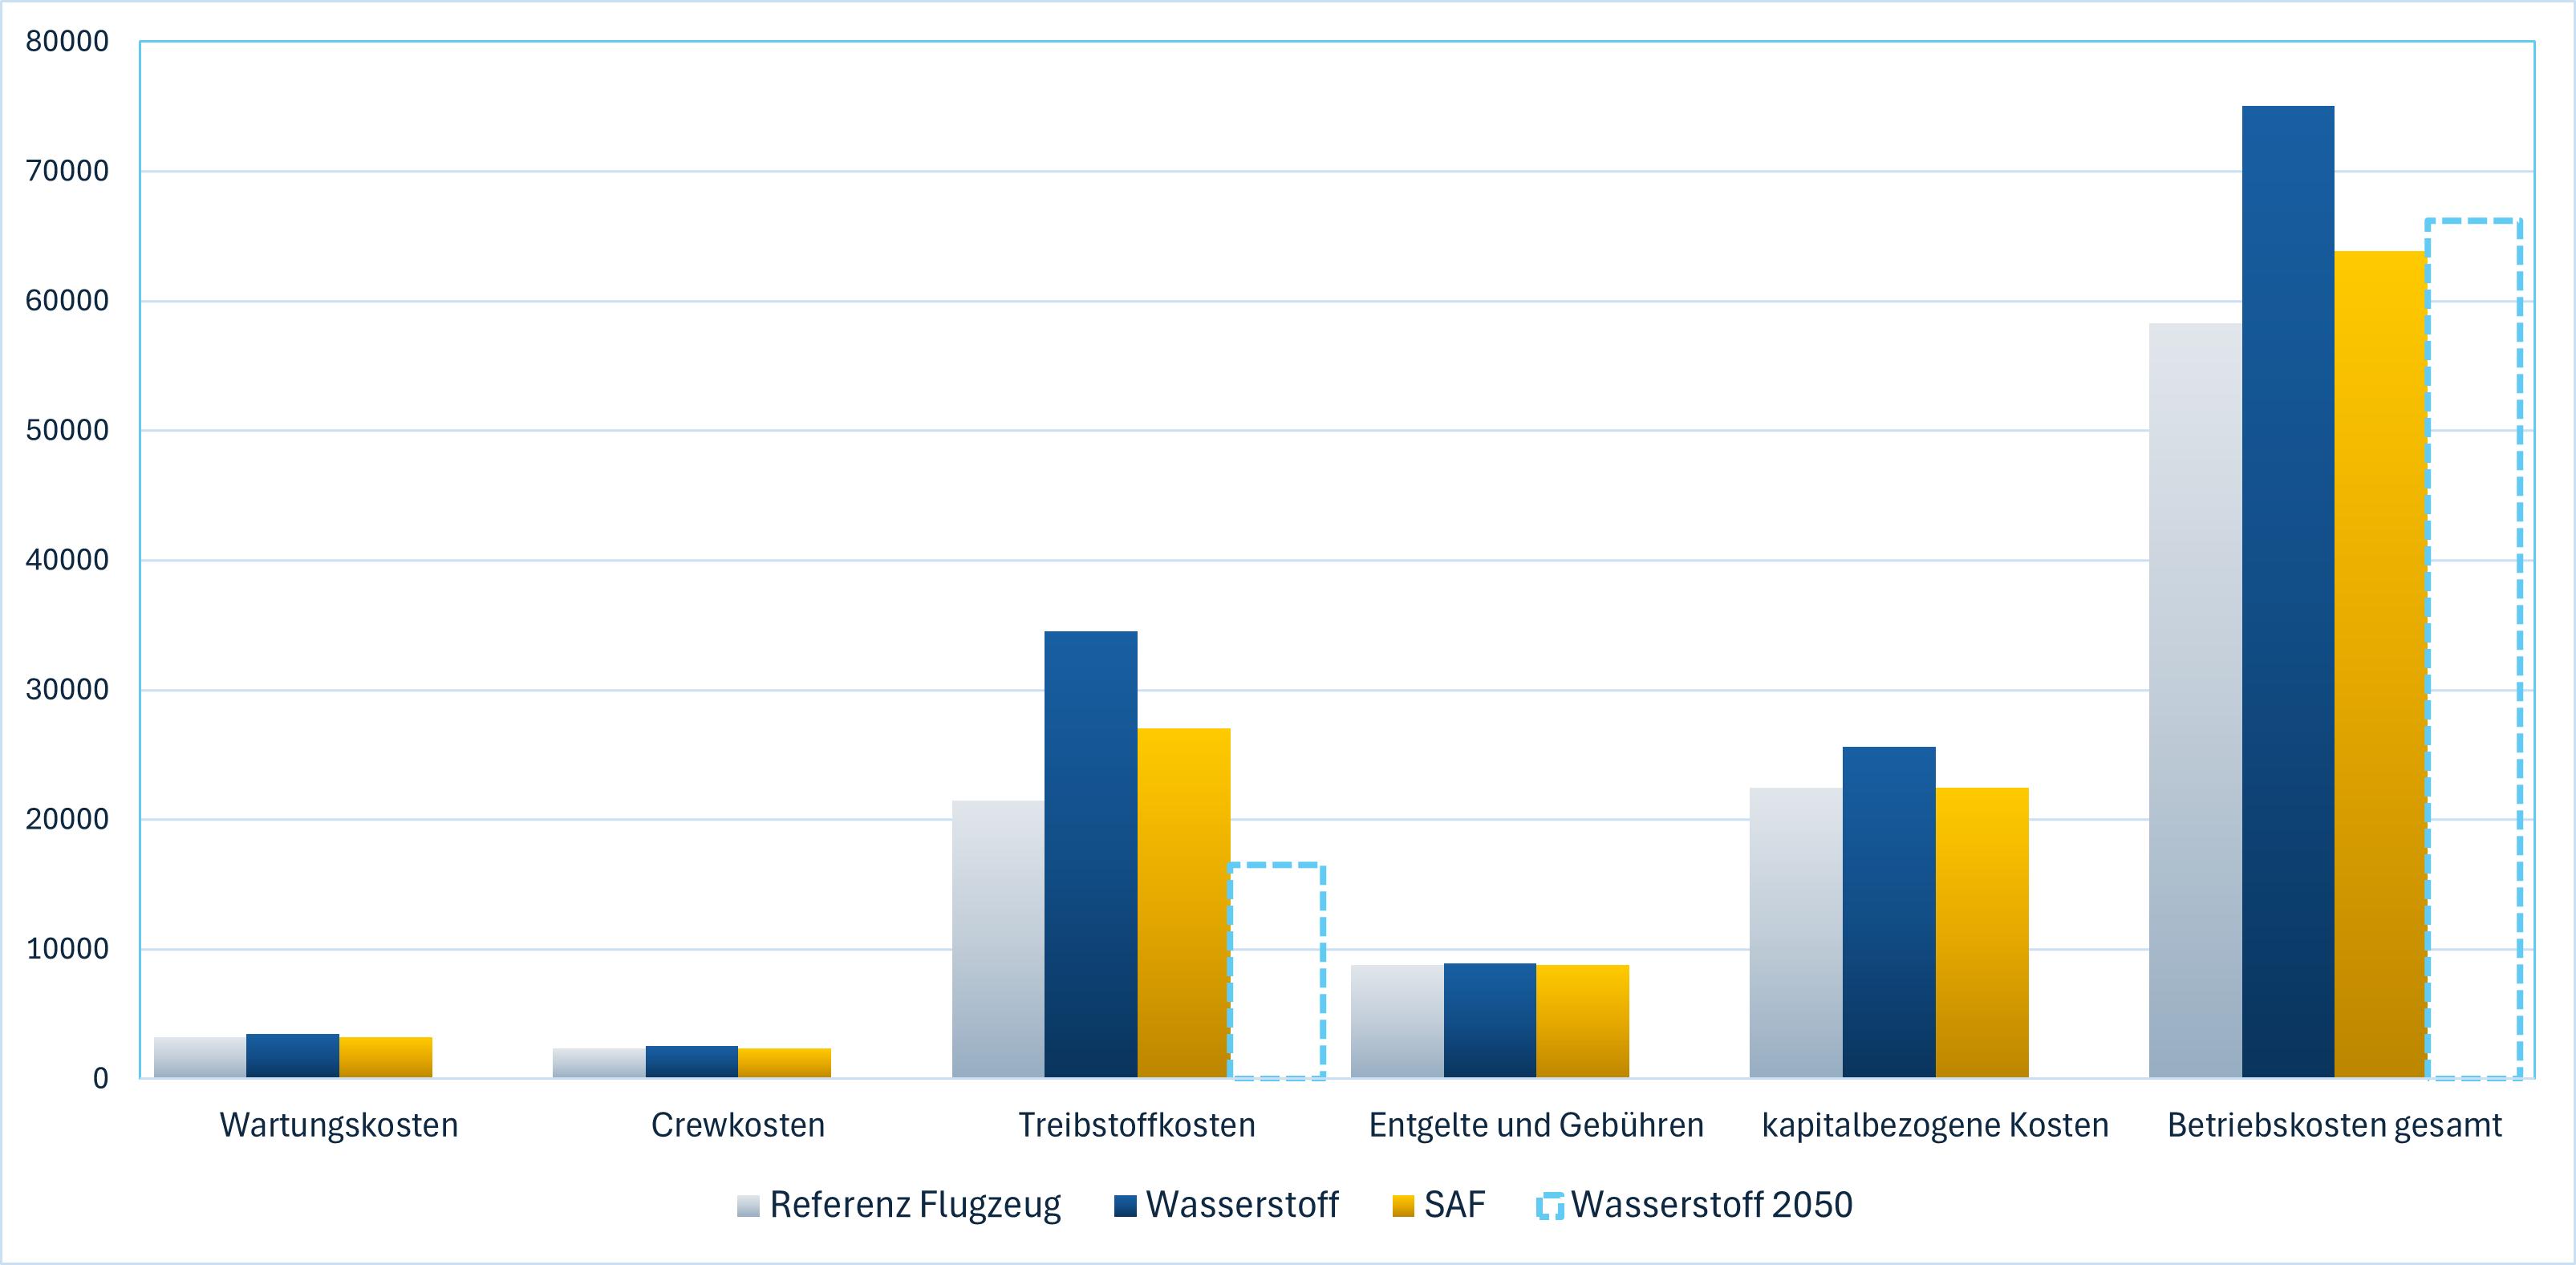
\includegraphics[width=0.9\linewidth]{Bilder/VergleichWA_SAF.png}
	\caption[Betriebskosten]{Vergleich der Referenz und Flugzeug mit der Wasserstoffantrieb und SAF für einen 6000 km Flug}
	\label{vergleichWA_Ref}
\end{figure}

Da die Treibstoffkosten einer der größten Teil in Ergebnissen ausmachen, wird der bedeutsame Parameter 
Treibstoffpreis für Sensitivitätsanalyse ausgewählt.

Werden Betriebskosten pro Passagierkilometer ausgerechnet und verglichen, haben die großen Flugzeuge geringere Kosten als die kleinen Flugzeuge.
Wie auch vorher resultiert wurde, haben hier konventionelle Treibstoffe den Vorteil unter den kleinen, als auch großen Flugzeugen.
